\documentclass[12pt,a4j,titlepage]{ltjsarticle}
\usepackage{semi}
\setcounter{tocdepth}{3}

\begin{document}
\begin{titlepage}
  \centering
    \vspace*{40truept}
    {\LARGE 2022年度 卒業論文}
    
    \vspace*{75truept}
    
    {\Huge 娯楽ゲームの教育的活用を推進する}
\vspace*{10truept}

    {\Huge Webサイトによる印象変化の調査}%論文タイトル

    \vspace{85truept}
    
    {\LARGE 指導教員 須田 宇宙 准教授}
    
    \vspace{60truept}
    
    {\LARGE 千葉工業大学 情報ネットワーク学科}
    
    \vspace{15truept}
    
    {\LARGE 須田研究室}
    
    \vspace{70truept}
    
    {\LARGE 1732008 氏名 五十嵐 美結 } % 氏名は消さない 学生番号 氏名 名前

    \vspace{70truept}
    
  \begin{flushright}

    \LARGE {提出日 2023年1月17日}
  
  \end{flushright}
\end{titlepage}
\date{}



\tableofcontents
\listoftables
\listoffigures
\clearpage
%1章
\section{緒言}\label{緒言}
%1章には,背景・問題点・目的を順番に書く.
%背景は,広く一般的な事柄を書いて,読む人に同意を抱かせつつ問題点につなぐ.
%問題点では,「〜という問題点がある」などのように,「問題」または「問題点」と言う単語を用いて,目的につなぐ.
%目的では,「そこで本研究では」から始めて,「〜を目的とする」で締める.
%以下は過去の卒業研究最終審査用の梗概の抜粋である.

%背景
近年,アクティブ・ラーニングとして授業活動にゲーミフィケーションといわれるゲームの娯楽性要素や,学習要素を盛り込んだシミュレーション等のゲーム(シリアスゲーム)を導入する動きが活発になってきている.
ゲーミフィケーションは楽しさ,目的意識,達成感の充実といったゲームの主要な要素を取り入れることによって授業への参加意欲や充実感の向上のために活用されている.
シリアスゲームはデジタルゲームの一種で主にコンピュータやタブレットなどを使用し,教育・医療・環境といった社会問題の解決を目的として,英語やプログラミング分野では実際に教育現場で活用されている.

%問題点
一方でデジタルゲームのうち,学習目的でない娯楽要素の多いゲームはゲーム依存症やゲーム脳等のイメージがあり,教育的なメリットや学習機会があることは周知されておらず自宅での学習の妨げになる等の悪い印象が広まってしまっている.

リサーチサービスを提供する会社である株式会社アスマークが2014年に行った「ゲームと子どもに関するアンケート調査」\cite{gameanq}では,ゲームで遊ぶことが子どもの発育・成長にどのような影響を与えると思うかという質問で悪い影響があると思うが半数を超え,中でもゲームが嫌いと答えた人の票数は77.2%という結果だった.
意見として前述のゲーム依存症になると考えやコミュニケーションや運動をしなくなる,ゲームで無駄な時間を過ごすより読書して知識・想像力を蓄えたほうが良いと考えがあった.
またこの問題によって保護者からプレイの制限をされることで,ゲームから得られる学習機会の損失になるという問題点がある.

そこで本研究では,学習を主目的としないデジタル娯楽ゲームの印象の改善とそれらの持つ教育的効果の周知を図るために,様々な娯楽ゲームの持つ教育的なメリットをタグ付けしたWebサイトの開発をし,それにより娯楽ゲームに教育効果や学習機会があることを理解したかを保護者へのアンケート調査を行い評価することを目的とする.
%2章
\section{ゲームについて}
\subsection{教育に活用されるゲームと娯楽ゲーム}
本稿で扱うゲームの種類は家庭用ゲーム機やパソコン,タブレット,スマートフォン等でプレイするデジタルゲームである.
またそのゲームは大まかに教育や学習目的のものと娯楽向けのゲームに分けることができる.

\subsubsection{教育に活用されるゲーム}\label{教育ゲーム}
\ref{緒言}で記述したシリアスゲームは学習や社会問題の解決のための専門的に開発されたゲームであり,海外の学校等の教育現場でギガタブ等のコンピュータを利用し導入されている.
例としてKONAMIが国連世界食料計画(WFP)と協力し発売した「Food Force」というゲームがあり,これは世界の飢餓撲滅のための食糧支援の活動が学べるものである.
プレイヤーはWFPの一員となり飢餓地域に食糧を届けるために物資を確保し輸送,緊急事態にも対処しながら実際に行われている支援をゲームを通して学び,考えを深めることができる.

シリアスゲームの他にも英語やプログラミングなどの学習のためのゲームや算数・数学の図形をシミュレーションするゲームなどがある.

\subsubsection{娯楽ゲーム}
本研究で主に扱っている娯楽ゲームは\ref{教育ゲーム}で述べたような学習が主目的のゲームとは違い,楽しさや達成感,感動,ストレス解消などを得ることが主目的のゲームで娯楽向けのものを指す.
例としてNintendoのスーパーマリオブラザーズやスプラトゥーン,あつまれどうぶつの森等が挙げられる.

\subsection{ゲームに関する課題}
インターネットやゲーム機器の技術発達に伴い使用者の低年齢化が進み,日常生活の一部や学習,娯楽に使用されるようになった.その反面,過剰な利用や有害な事物に触れることが増えている.
ゲームに関しては過剰利用によるゲーム依存やゲーム脳の問題があり,ニュース等で取り上げられるなどして問題視されている.

\subsubsection{ゲーム依存・ゲーム脳}
ゲーム依存症は正式に「インターネット・ゲーム依存症」や「ゲーム障害」と言い,インタターネットやゲームをする時間が長くなり日常生活に支障を来し,他のことに興味を失ったり考えることが限定的になったりする症状が出る病気である.
これにより家族や友人関係が良好でなくなり健康にも害が生じる例がある.

ゲーム脳は日本大学の教授である森昭雄氏が2002年に出版した「ゲーム脳の恐怖」\cite{ゲーム脳の恐怖}で提示された造語で,コンピュータゲームや携帯電話・パソコンを操作することにより脳に悪影響を与えるというものである.
ただ,当時の実験で使用した計測器等が記されておらず信憑性に欠けることやゲーム脳を証明する論文がないことから疑問視されているが,テレビやインターネット等のマスメディアで肯定的に取り上げられたため\cite{ゲーム脳メディア}世間に広まった.

\subsubsection{香川県ネット・ゲーム依存症対策条例}

%3章
\section{アンケート調査}\label{アンケート調査}
\ref{Webサイトについて}章で述べるサイトを対象者が閲覧した後の娯楽ゲームの教育的なメリットへの理解とイメージの変化を調査するためにアンケートを行った.

\subsection{調査概要}
調査対象である小中学生の子を持つ保護者10人に調査を行った.対象者の情報については子の年齢(表\ref{table:情報})やゲームをプレイする機器の所持状況の他に回答者や子が週にゲームをプレイする頻度や好き嫌い,回答者が子供の頃のゲームプレイの頻度を収集した.

\begin{table}[h]
 \caption{対象者の子どもの年齢分布}
 \label{table:情報}
 \small
 \centering
  \begin{tabular}{lrrrrrrrr}
  \hline
   子の年齢 & 未就学児 & 小学1,2年 & 3,4年 & 5,6年 & 中学1年 & 2年 & 3年 & 高校以上\\
   (人)& 2 & 3 & 2 & 4 & 3 & 1 & 2 & 0\\
   \hline
  \end{tabular}
\end{table}

\begin{figure}[h]
 \begin{center}
  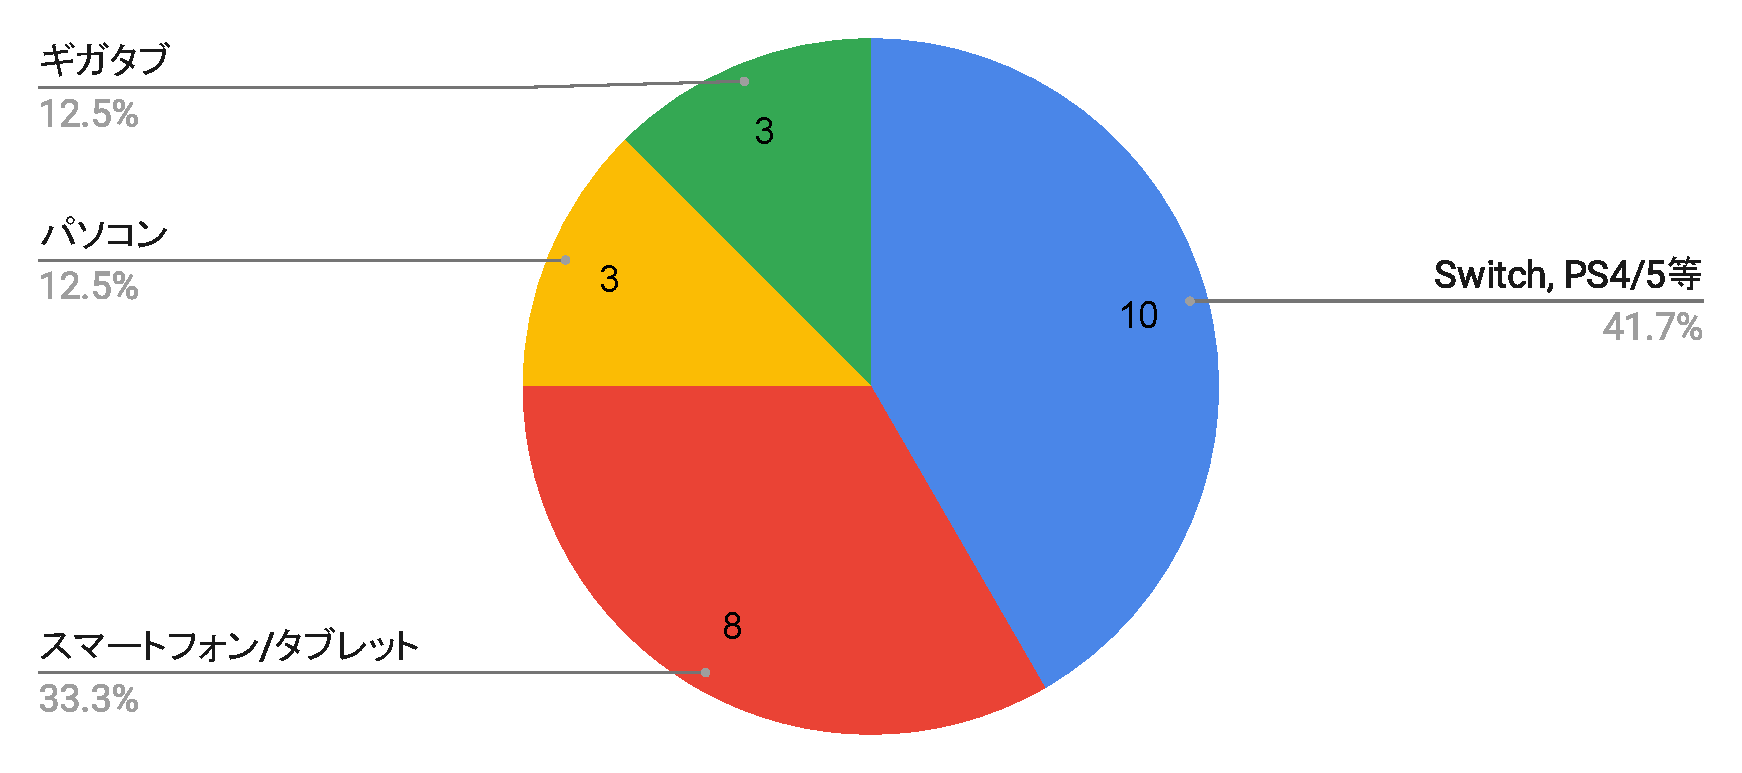
\includegraphics[keepaspectratio, scale=0.4]{chart1.pdf}
 \end{center}
 \caption{子どもも使用できる家庭用のゲーム機,スマートフォン,タブレット等はあるか}
 \label{fig:ゲーム所持}
\end{figure}

ゲーム機器の所持状況について(\ref{fig:ゲーム所持})はNintendo SwitchやPlayStation4/5といった家庭用ゲーム機やスマートフォン・タブレット端末,またパソコンや学校から配布されたタブレット端末・パソコンであるギガタブを選択肢とした.
子どもの対象が小中学生のためか家庭用ゲーム機が10票,スマートフォン・タブレットが8票と多くを占めた.

\begin{figure}[h]
 \begin{center}
  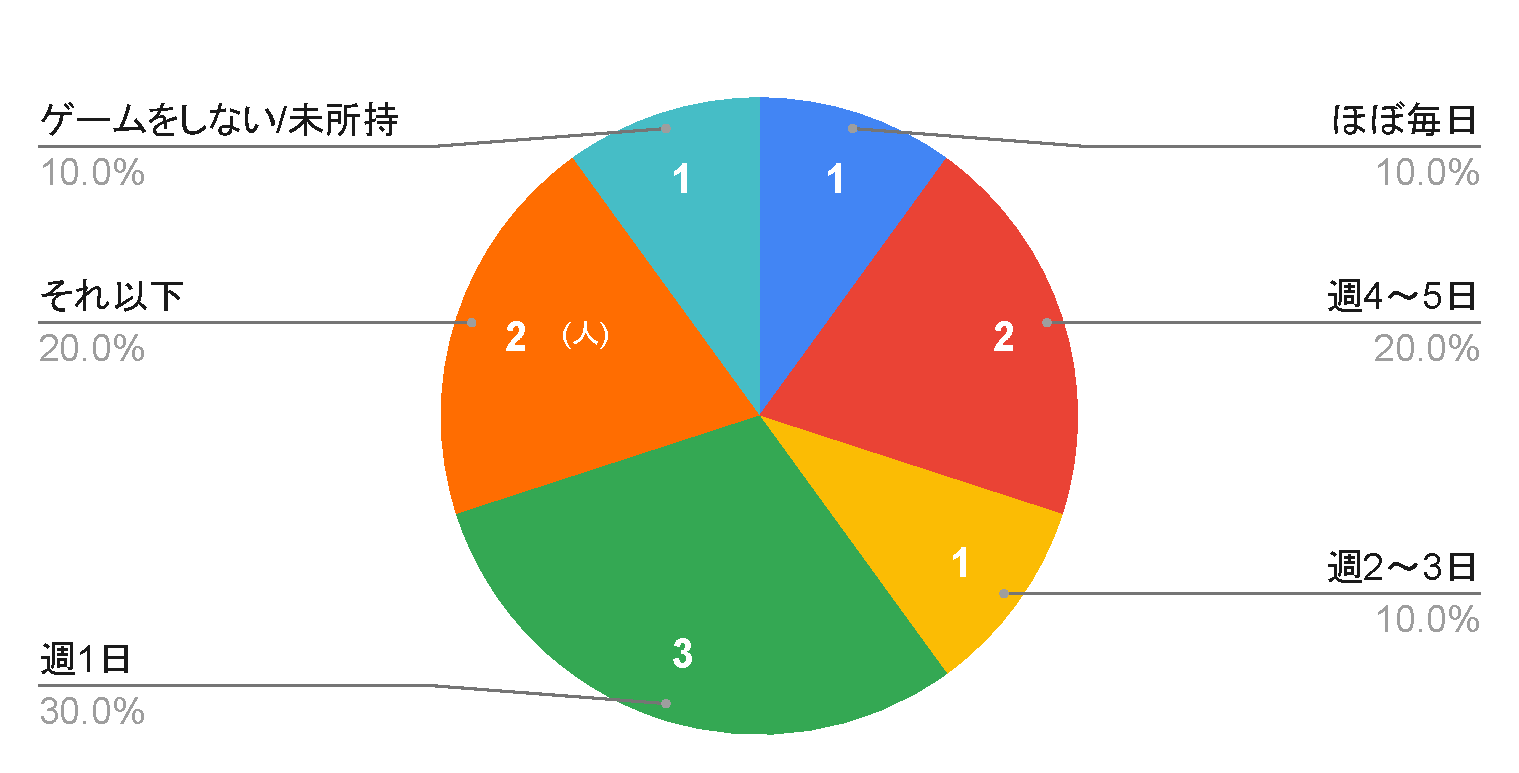
\includegraphics[keepaspectratio, scale=0.4]{chart2.pdf}
 \end{center}
 \caption{回答者はどれくらいの頻度でゲームをプレイするか}
 \label{fig:プレイ頻度(回答者)}
\end{figure}

\begin{figure}[h]
 \begin{center}
  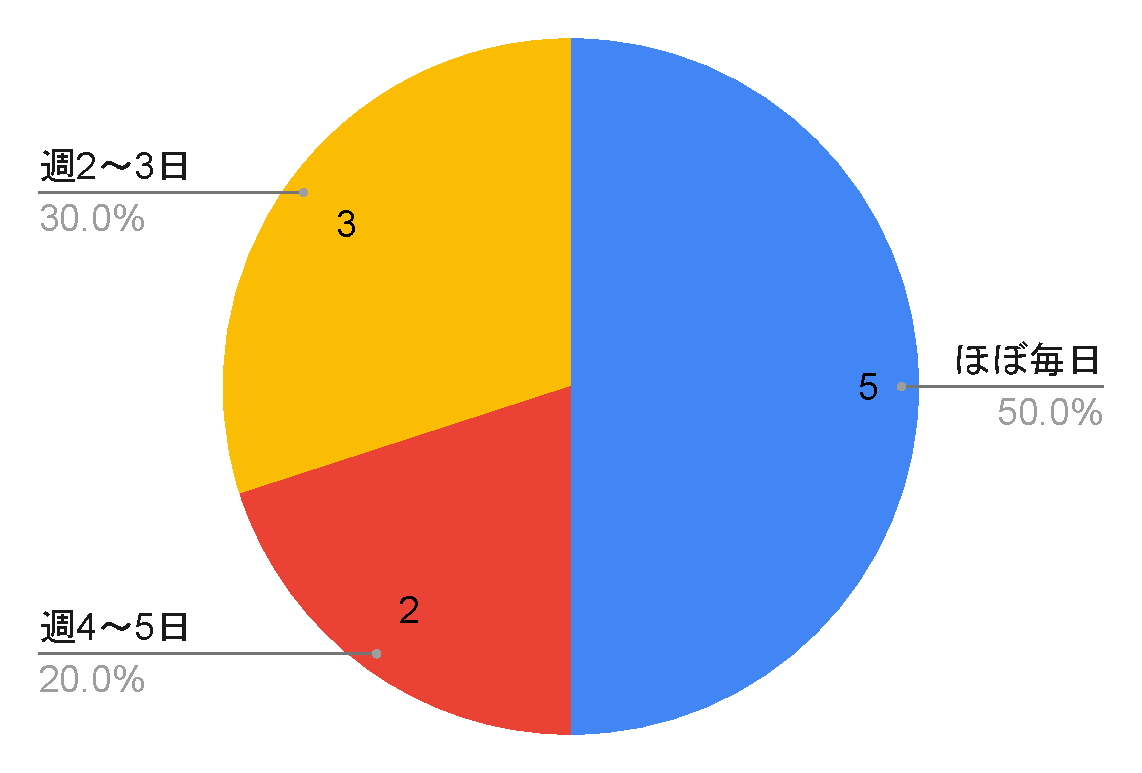
\includegraphics[keepaspectratio, scale=0.4]{chart3.pdf}
 \end{center}
 \caption{子どもはどれくらいの頻度でゲームをプレイするか}
 \label{fig:プレイ頻度(子ども)}
\end{figure}

回答者と子どものゲームのプレイ頻度についての質問では,回答者である保護者は週1日と週4~5日プレイするという人が多く頻度はそれほど高くなかったが,子どものプレイ頻度はほぼ毎日するという人が半数を占めそれ以外も高頻度でプレイしていることが分かった.

\begin{figure}[h]
 \begin{center}
  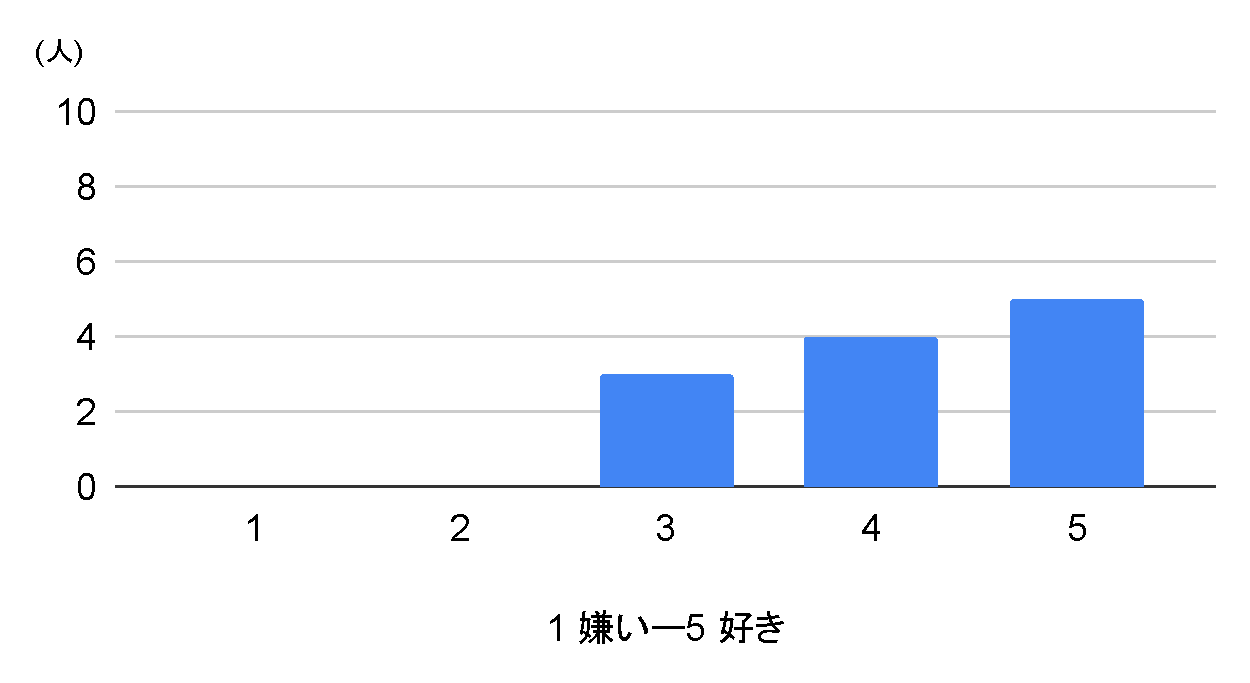
\includegraphics[keepaspectratio, scale=0.5]{chart4.pdf}
 \end{center}
 \caption{回答者はゲームが好きか}
 \label{fig:好き嫌い(回答者)}
\end{figure}

\begin{figure}[h]
 \begin{center}
  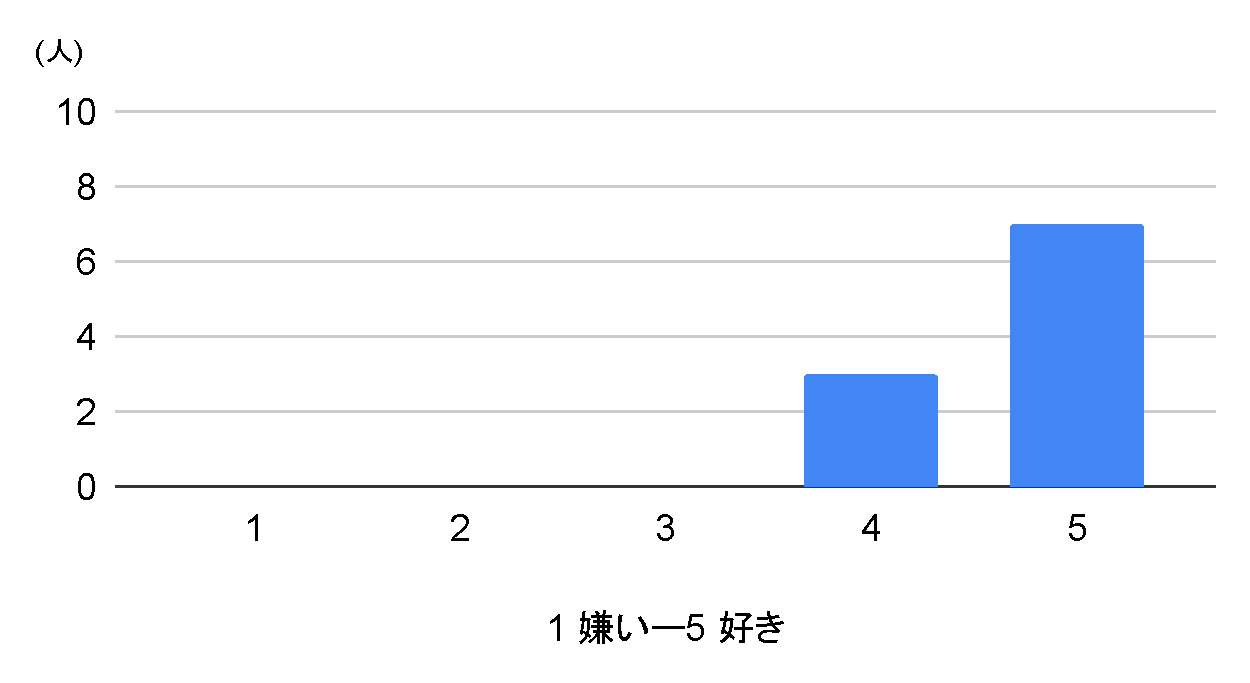
\includegraphics[keepaspectratio, scale=0.5]{chart5.pdf}
 \end{center}
 \caption{子どもはゲームが好きか}
 \label{fig:好き嫌い(子ども)}
\end{figure}

回答者と子どもがゲームが好きかという質問では回答者である保護者は嫌いという回答はなくどちらでもないから好きである傾向にあった.
回答者のプレイ頻度(図\ref{fig:プレイ頻度(回答者)})ではあまりゲームをしないという人もいたが,ゲームが嫌いという傾向にないことが分かった.

子どもはやや好きが3票,好きが7票という結果になった.
図\ref{fig:プレイ頻度(子ども)}の子どものゲームのプレイ頻度の傾向から見てもゲームが好きである人が多いことは容易に窺える.

\begin{figure}[h]
 \begin{center}
  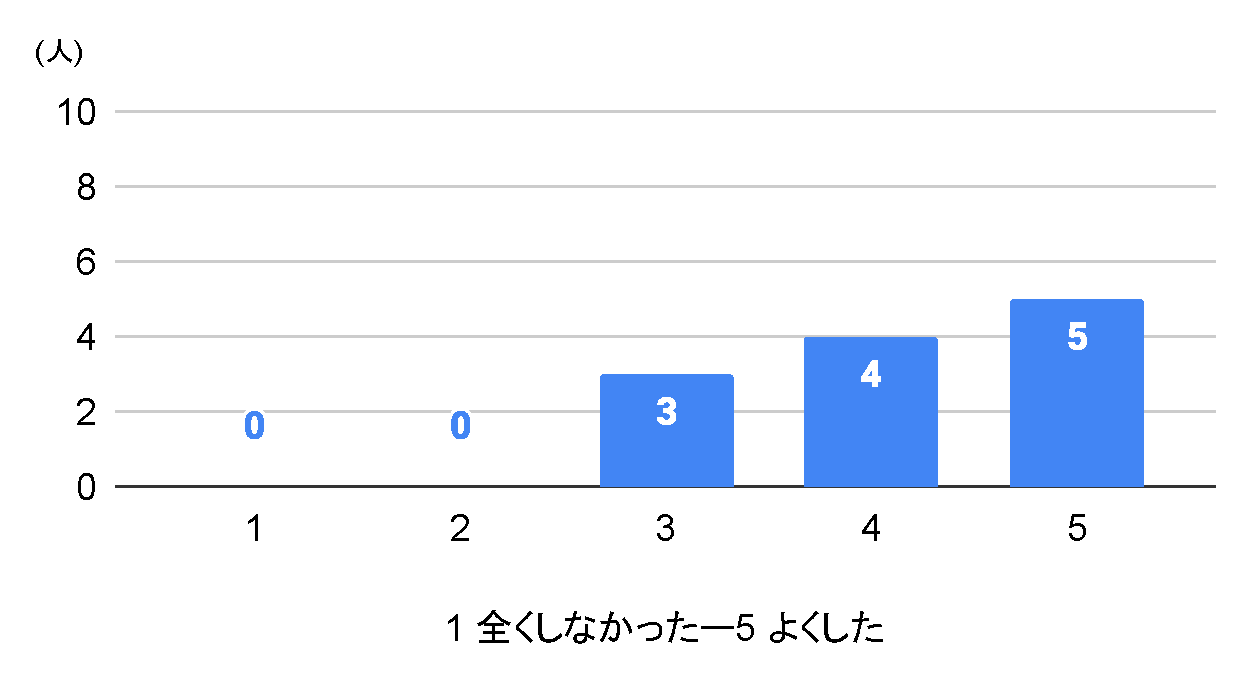
\includegraphics[keepaspectratio, scale=0.5]{chart6.pdf}
 \end{center}
 \caption{子どもの頃ゲームで遊ぶことはあったか}
 \label{fig:子どものころ}
\end{figure}

\subsection{調査項目}\label{調査項目}
調査として回答者にゲームが子どもに与える影響について全体的にどのようなイメージを持っているかを聞き,さらにその詳細として勉強面,友人関係・コミュニケーション,感性,知識・教養,時間管理,健康面の影響についてのイメージと読書やスポーツといった他の趣味活動とのメリットの比較について,Webサイトを見る前と見た後について調査した.(表\ref{table:anque})
項目については株式会社アスマークが行ったアンケート調査\cite{gameanq}の意見記述の一部(\ref{table:asmarqanque})を参考に,iはa,b,ⅱはc,d,ⅲはe,ⅳはd,vはb,f,ⅵはg,ⅶはhというようにゲームが子どもにとって良い悪いに関わらず影響を与えると考えられているものを扱った.

さらにアンケートの最後部に,作成した記事に書かれたゲームについてのメリットが今後の子どもの発育・成長に影響があると思うかという質問と意見記述の欄を設けた.

\begin{table}[h]
 \caption{アンケート}
 \label{table:anque}
 \small
 \centering
  \begin{tabular}{l}
  \hline
  子に与える影響について \\
   \hline \hline
   ⅰ.勉強面 \\
   ⅱ.友人関係,コミュニケーション\\
   ⅲ.感性\\
   ⅳ.知識,教養 \\
   ⅴ.時間管理   \\
   ⅵ.健康面 \\
   ⅶ.読書・スポーツ等他の趣味とのメリットの比較 \\
   \hline
  \end{tabular}
\end{table}

\begin{table}[h]
 \caption{アスマークによるアンケート調査の意見記述(一部抜粋)}
 \label{table:asmarqanque}
 \small
 \centering
  \begin{tabular}{l}
  \hline
   a. 最近では勉強できるソフトもたくさんあって,自分自身役に立っている\\
   b. 学習時間や運動の時間,睡眠時間を削ることにつながる \\
   c. 現実から逃避され,人とのコミュニケーションがなくなる \\
   d. 友人関係の形成,コミュニケーションツール,知識の習得と言った面ではプラスの作用もある \\
   e. 感性が豊かになるとは思うが,結局はムダな時間ではあるのでバランスが大事だとは思う \\
   f. 遊ぶ時間などのルールをきっちりと決め,親の管理の上でやらせなければ無制限にやることになる\\
   g. 外で身体を動かす遊びを全くしなくなった.動かないので太りやすい \\
   h. 読書して知識や想像力を蓄えたほうが良い \\
   \hline
  \end{tabular}
\end{table}

%4章
\section{アンケート結果}
\ref{調査項目}の図\ref{table:anque}で述べたそれぞれのアンケート項目の結果とその評価について述べる.

\subsection{結果}
ああああああああああああああああああああああああああああああああああああああ

ああああああああああああああ

\begin{figure}[h]
 \begin{center}
  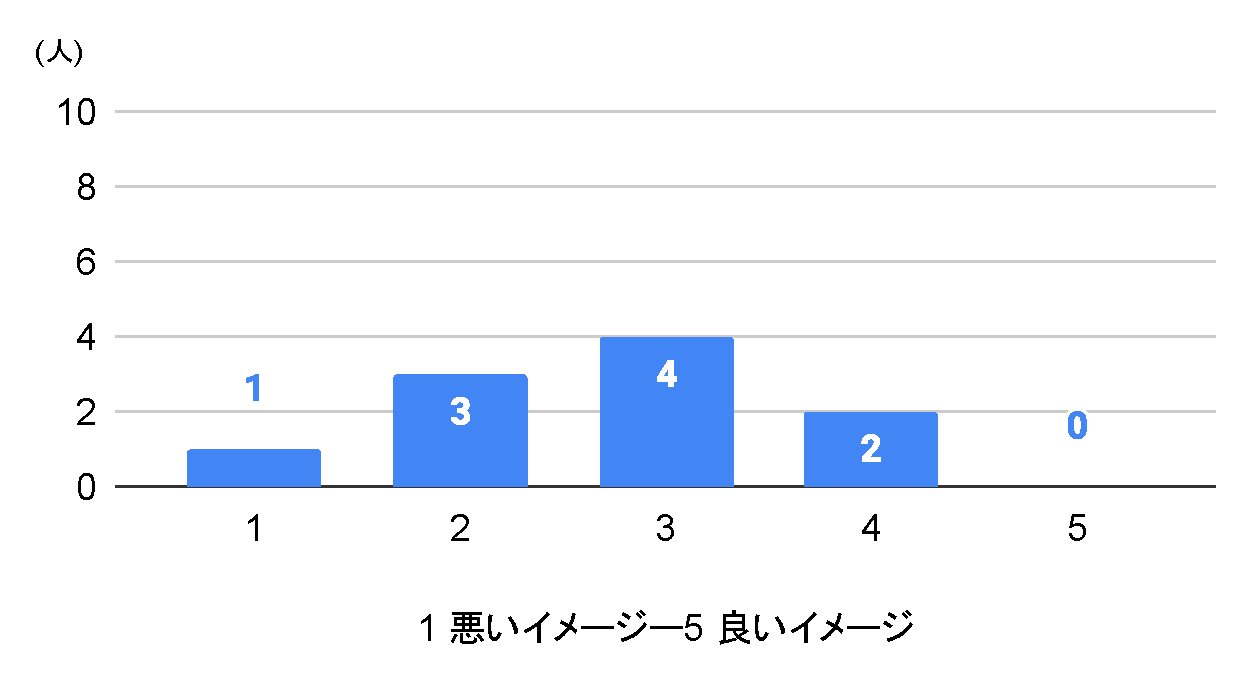
\includegraphics[keepaspectratio, scale=0.5]{印象前.pdf}
 \end{center}
 \caption{サイトを見る前はゲームが子どもの発育・成長へ与える影響に対して大まかにどのようなイメージを持っていたか}
 \label{fig:見る前印象}
\end{figure}

\begin{figure}[h]
 \begin{center}
  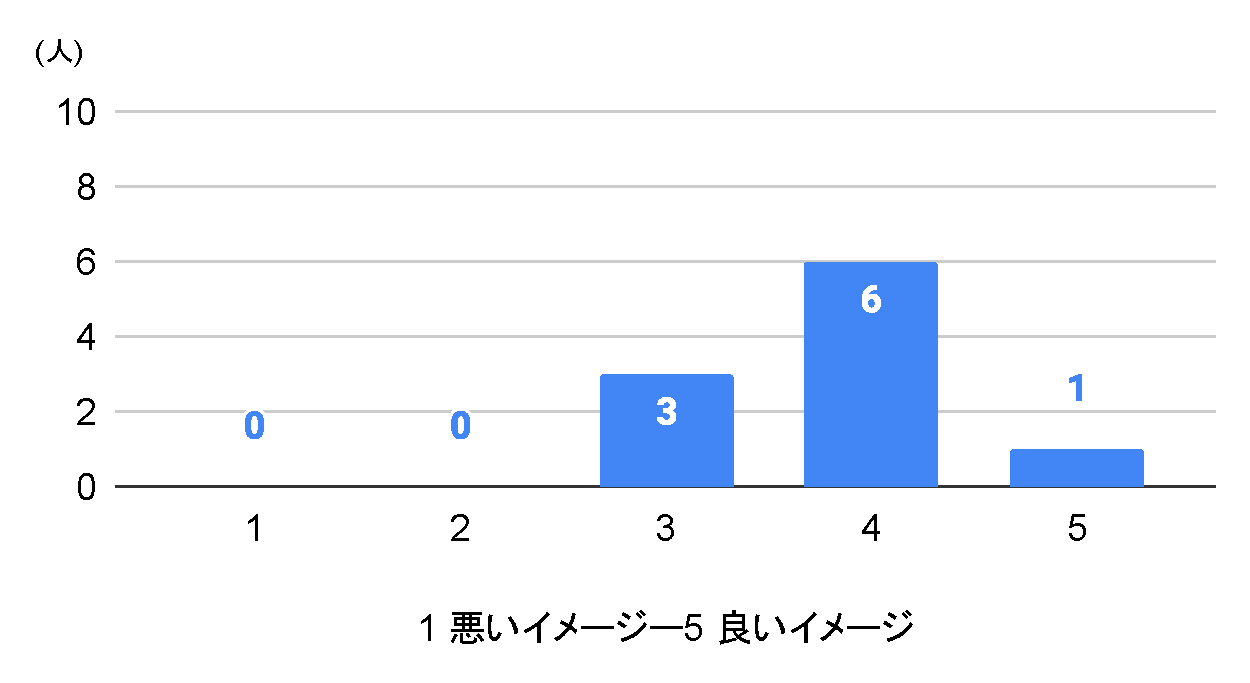
\includegraphics[keepaspectratio, scale=0.5]{印象後.pdf}
 \end{center}
 \caption{サイトを見た後はゲームが子どもの発育・成長へ与える影響に対して大まかにどのようなイメージを持ったか}
 \label{fig:見た後印象}
\end{figure}

\begin{figure}[h]
 \begin{center}
  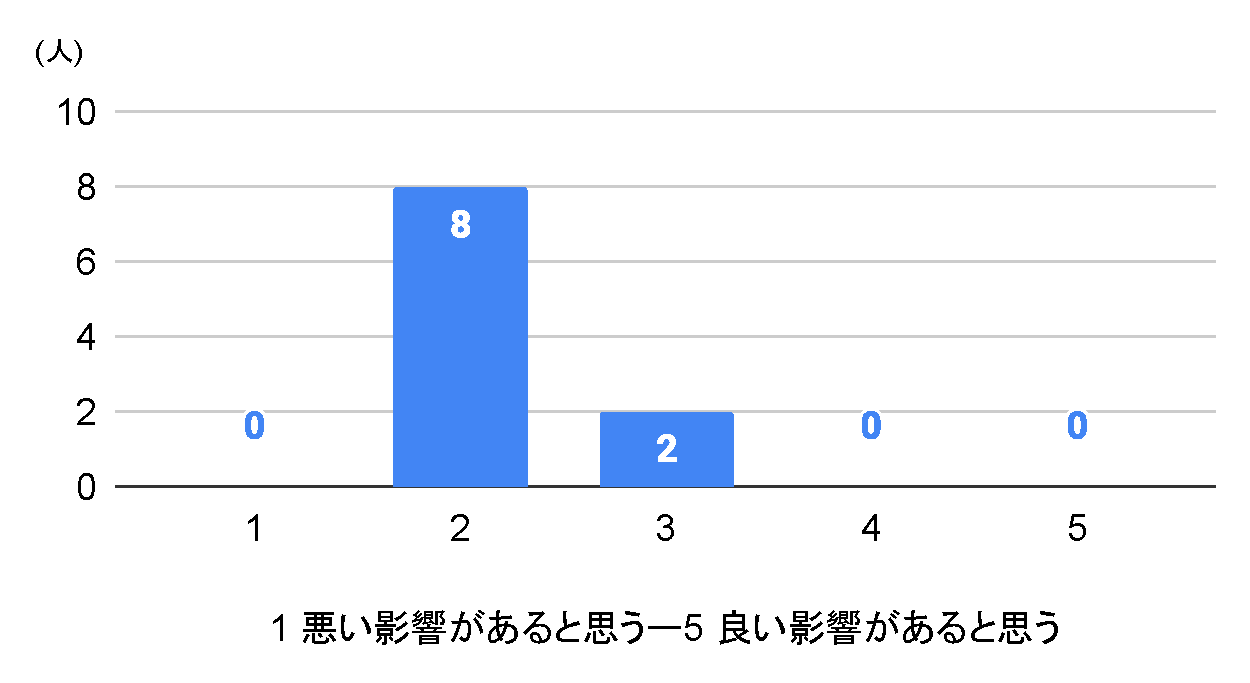
\includegraphics[keepaspectratio, scale=0.5]{勉強前.pdf}
 \end{center}
 \caption{ゲームが勉強面に与える影響についてどのように考えていたか}
 \label{fig:勉強前}
\end{figure}

\begin{figure}[h]
 \begin{center}
  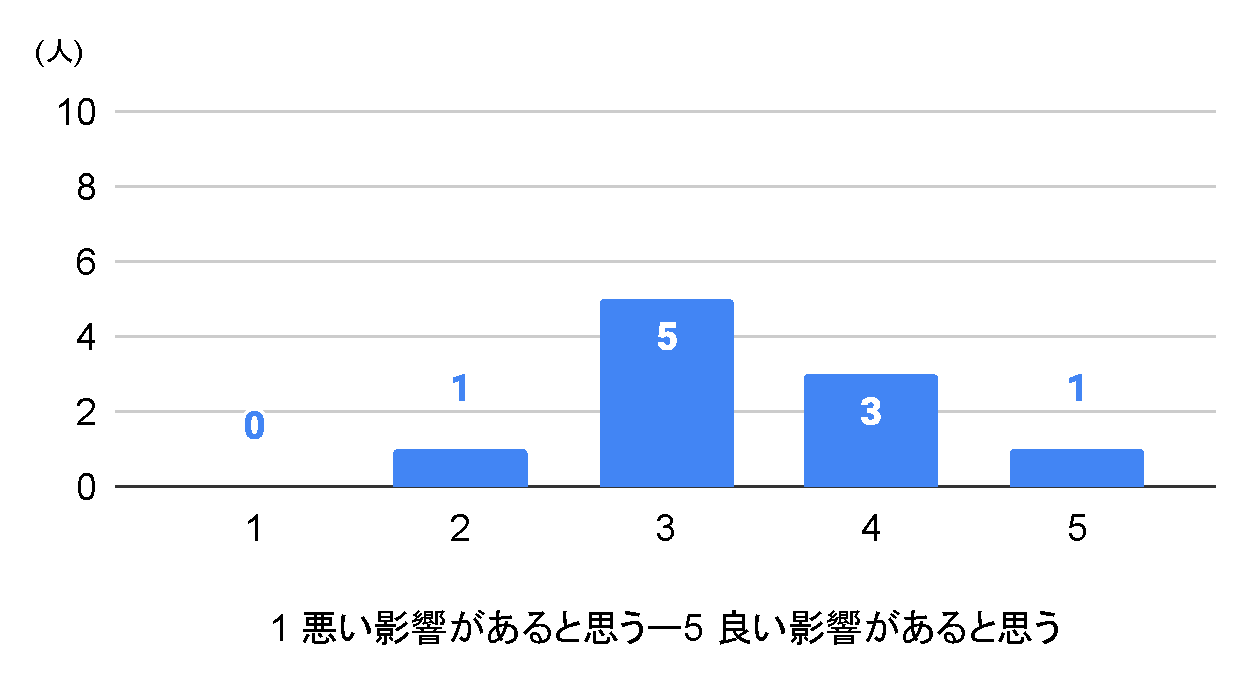
\includegraphics[keepaspectratio, scale=0.5]{勉強後.pdf}
 \end{center}
 \caption{ゲームが勉強面に与える影響についてどのように考えたか}
 \label{fig:勉強後}
\end{figure}

\begin{figure}[h]
 \begin{center}
  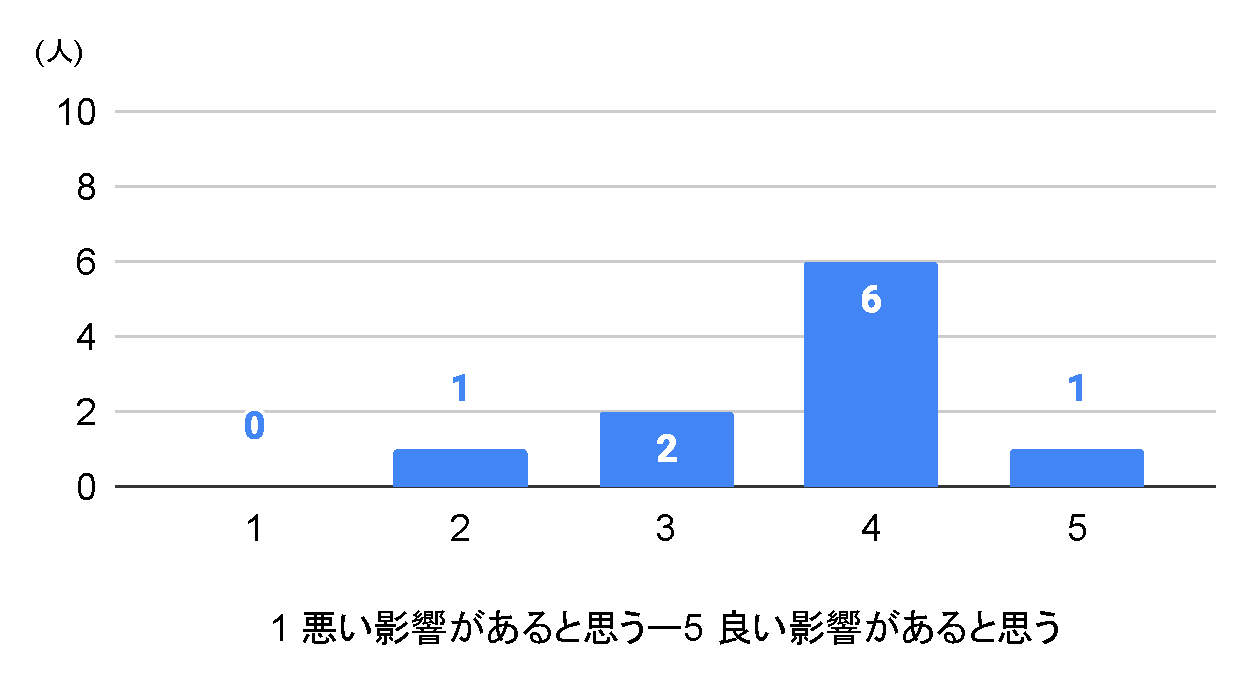
\includegraphics[keepaspectratio, scale=0.5]{コミュ前.pdf}
 \end{center}
 \caption{ゲームが友人関係・コミュニケーションに与える影響についてどのように考えていたか}
 \label{fig:コミュ前}
\end{figure}

\begin{figure}[h]
 \begin{center}
  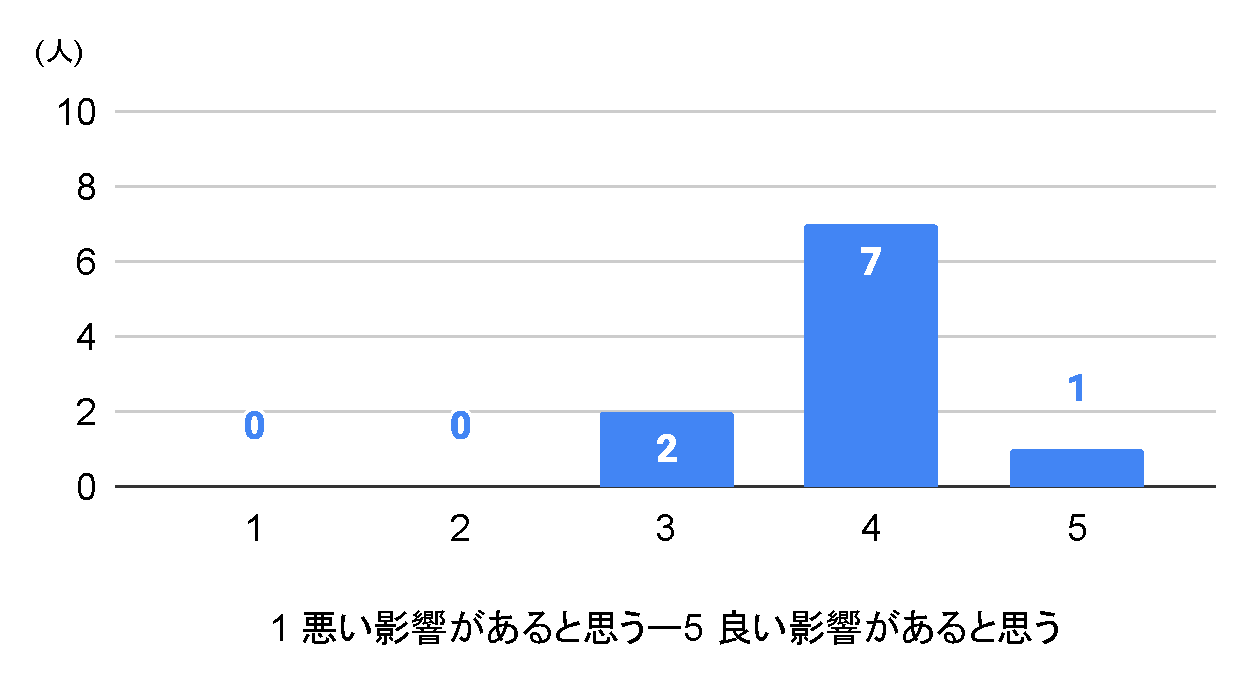
\includegraphics[keepaspectratio, scale=0.5]{コミュ後.pdf}
 \end{center}
 \caption{ゲームが友人関係・コミュニケーションに与える影響についてどのように考えたか}
 \label{fig:コミュ後}
\end{figure}

\begin{figure}[h]
 \begin{center}
  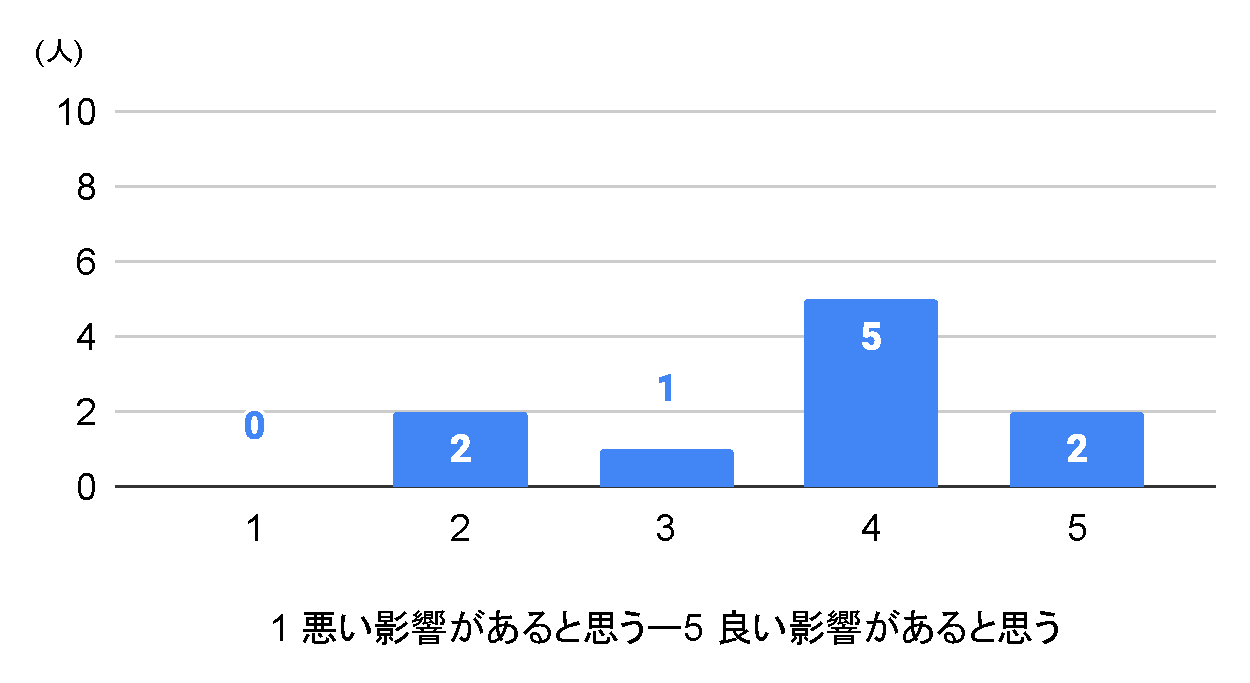
\includegraphics[keepaspectratio, scale=0.5]{感性前.pdf}
 \end{center}
 \caption{ゲームが感性に与える影響についてどのように考えていたか}
 \label{fig:感性前}
\end{figure}

\begin{figure}[h]
 \begin{center}
  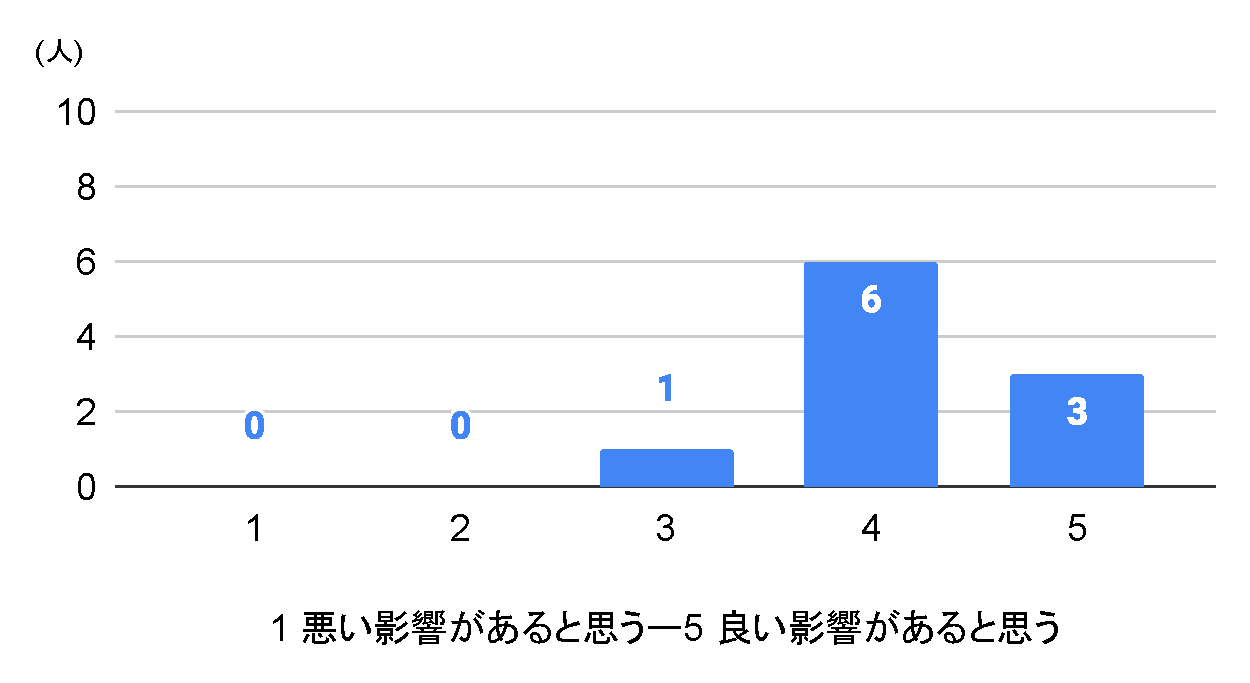
\includegraphics[keepaspectratio, scale=0.5]{感性後.pdf}
 \end{center}
 \caption{ゲームが感性に与える影響についてどのように考えたか}
 \label{fig:感性後}
\end{figure}

\begin{figure}[h]
 \begin{center}
  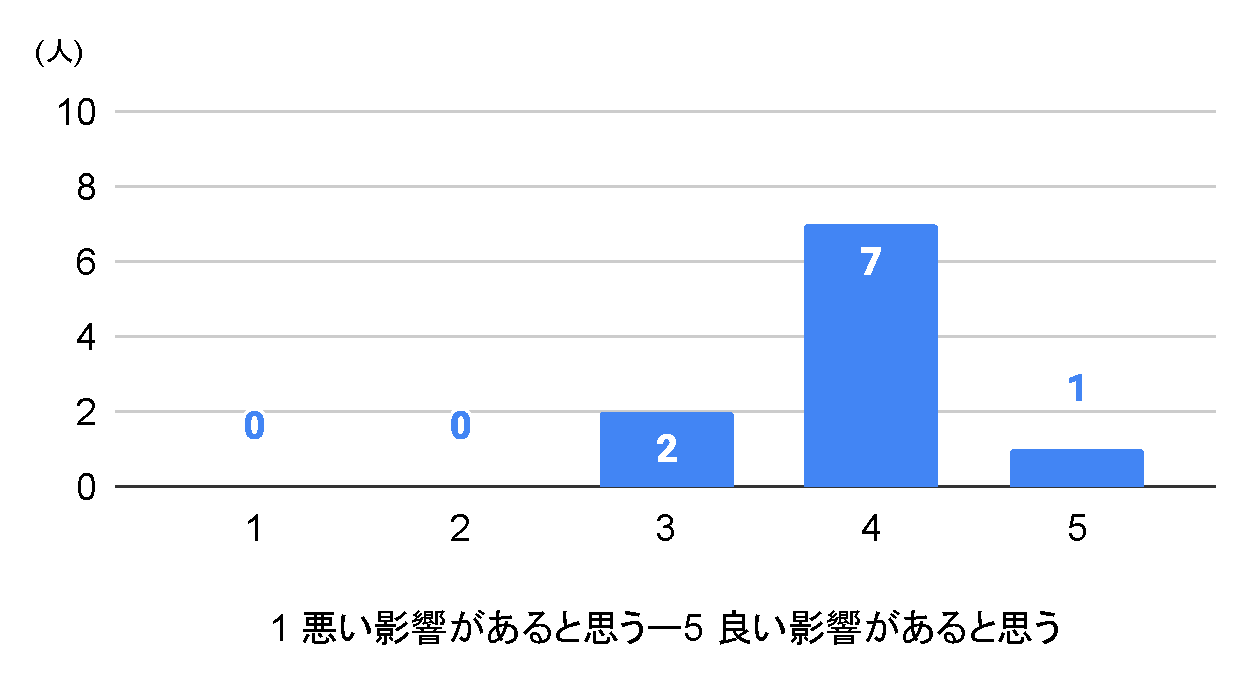
\includegraphics[keepaspectratio, scale=0.5]{知識前.pdf}
 \end{center}
 \caption{ゲームが知識・教養に与える影響についてどのように考えていたか}
 \label{fig:知識前}
\end{figure}

\begin{figure}[h]
 \begin{center}
  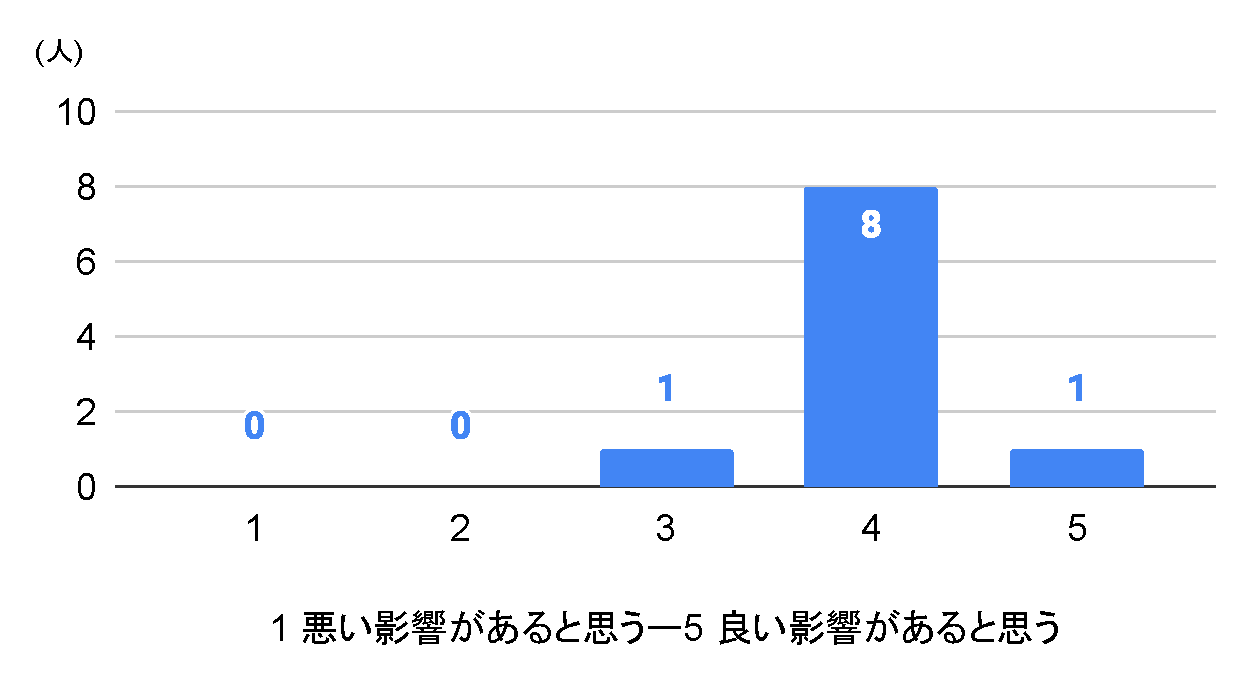
\includegraphics[keepaspectratio, scale=0.5]{知識後.pdf}
 \end{center}
 \caption{ゲームが知識・教養に与える影響についてどのように考えたか}
 \label{fig:知識後}
\end{figure}

\begin{figure}[h]
 \begin{center}
  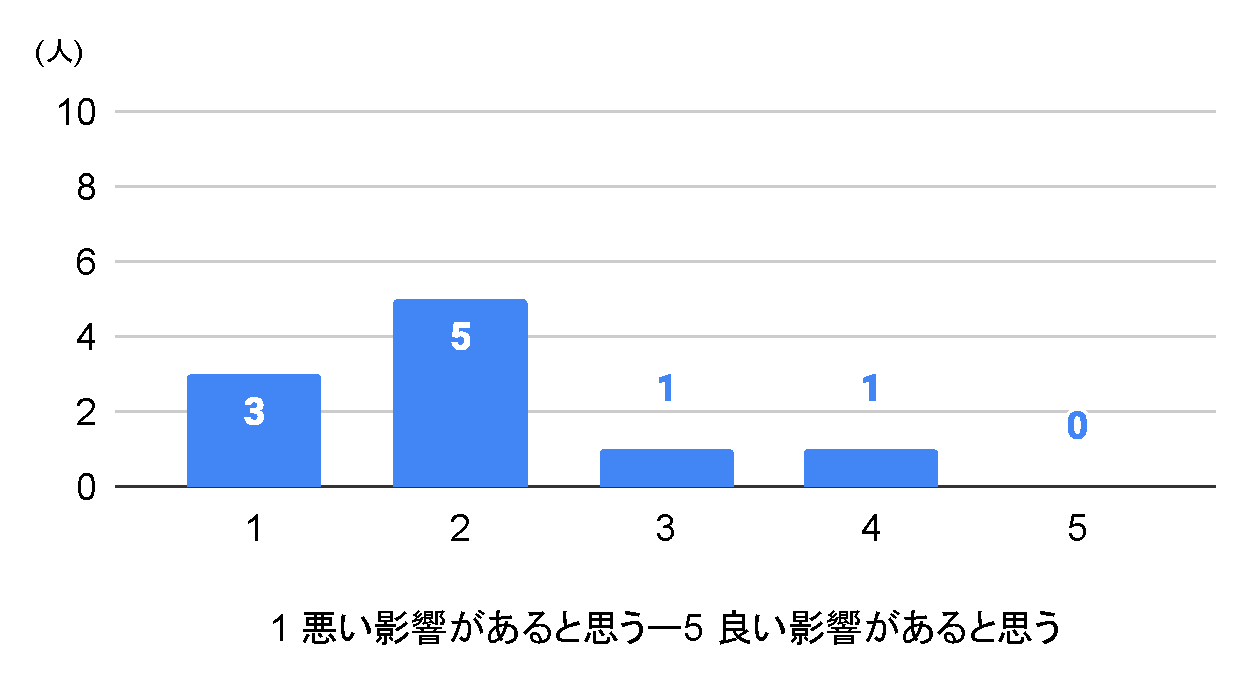
\includegraphics[keepaspectratio, scale=0.5]{時間前.pdf}
 \end{center}
 \caption{ゲームが時間管理に与える影響についてどのように考えていたか}
 \label{fig:時間前}
\end{figure}

\begin{figure}[h]
 \begin{center}
  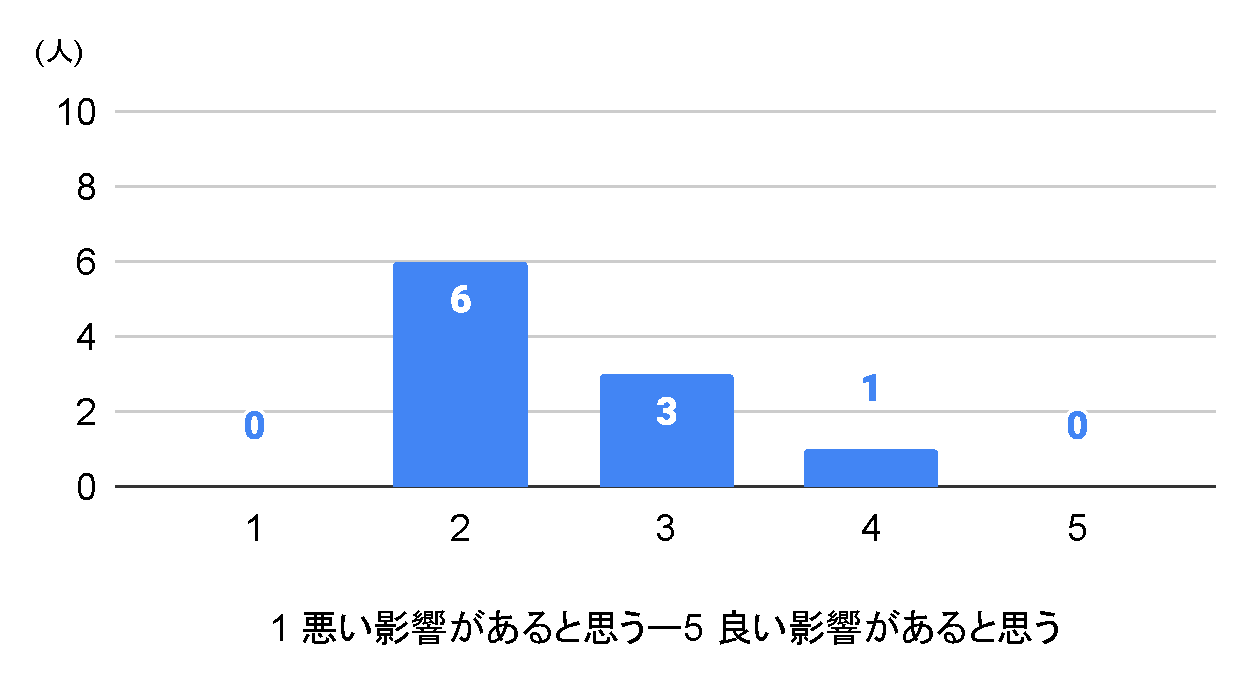
\includegraphics[keepaspectratio, scale=0.5]{時間後.pdf}
 \end{center}
 \caption{ゲームが時間管理に与える影響についてどのように考えたか}
 \label{fig:時間後}
\end{figure}

\begin{figure}[h]
 \begin{center}
  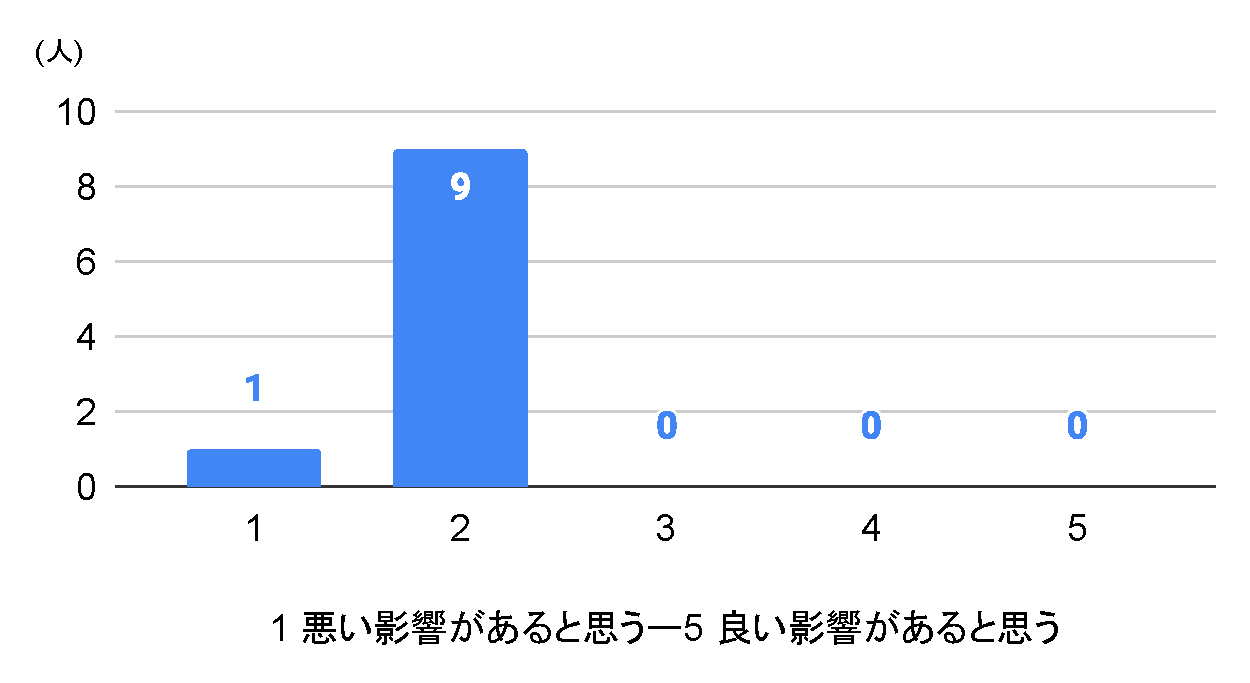
\includegraphics[keepaspectratio, scale=0.5]{健康前.pdf}
 \end{center}
 \caption{ゲームが健康面に与える影響についてどのように考えていたか}
 \label{fig:健康前}
\end{figure}

\begin{figure}[h]
 \begin{center}
  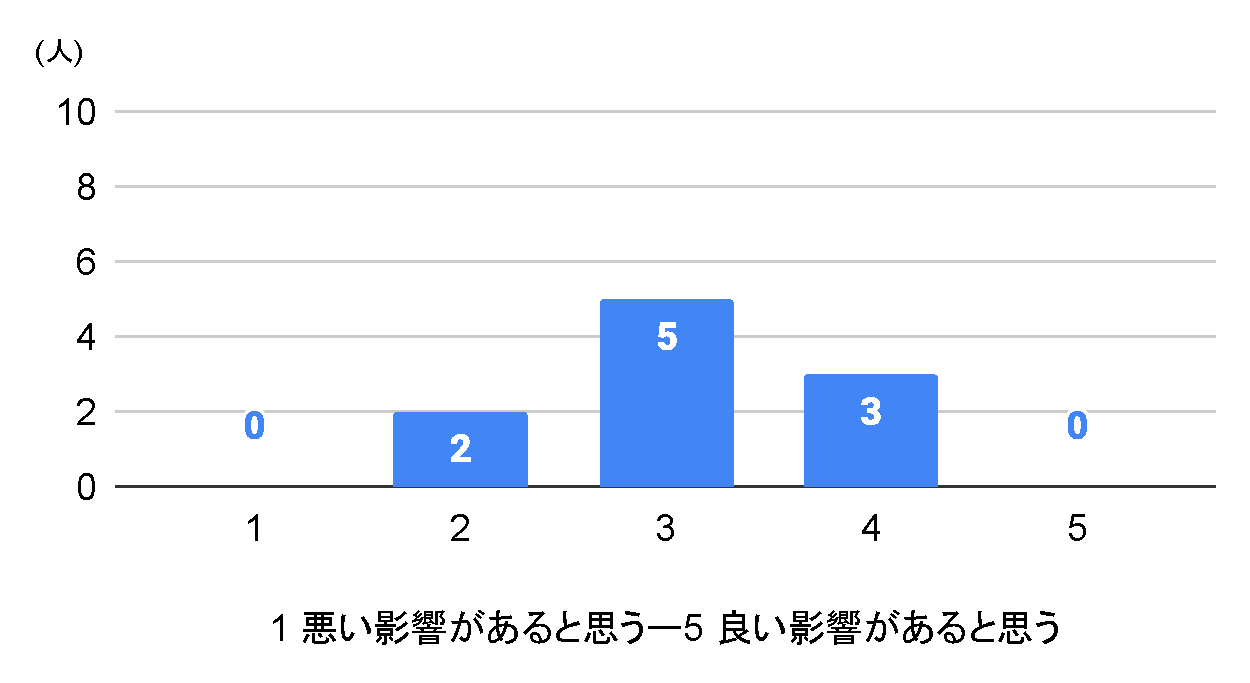
\includegraphics[keepaspectratio, scale=0.5]{健康後.pdf}
 \end{center}
 \caption{ゲームが健康面に与える影響についてどのように考えたか}
 \label{fig:健康後}
\end{figure}

\begin{figure}[h]
 \begin{center}
  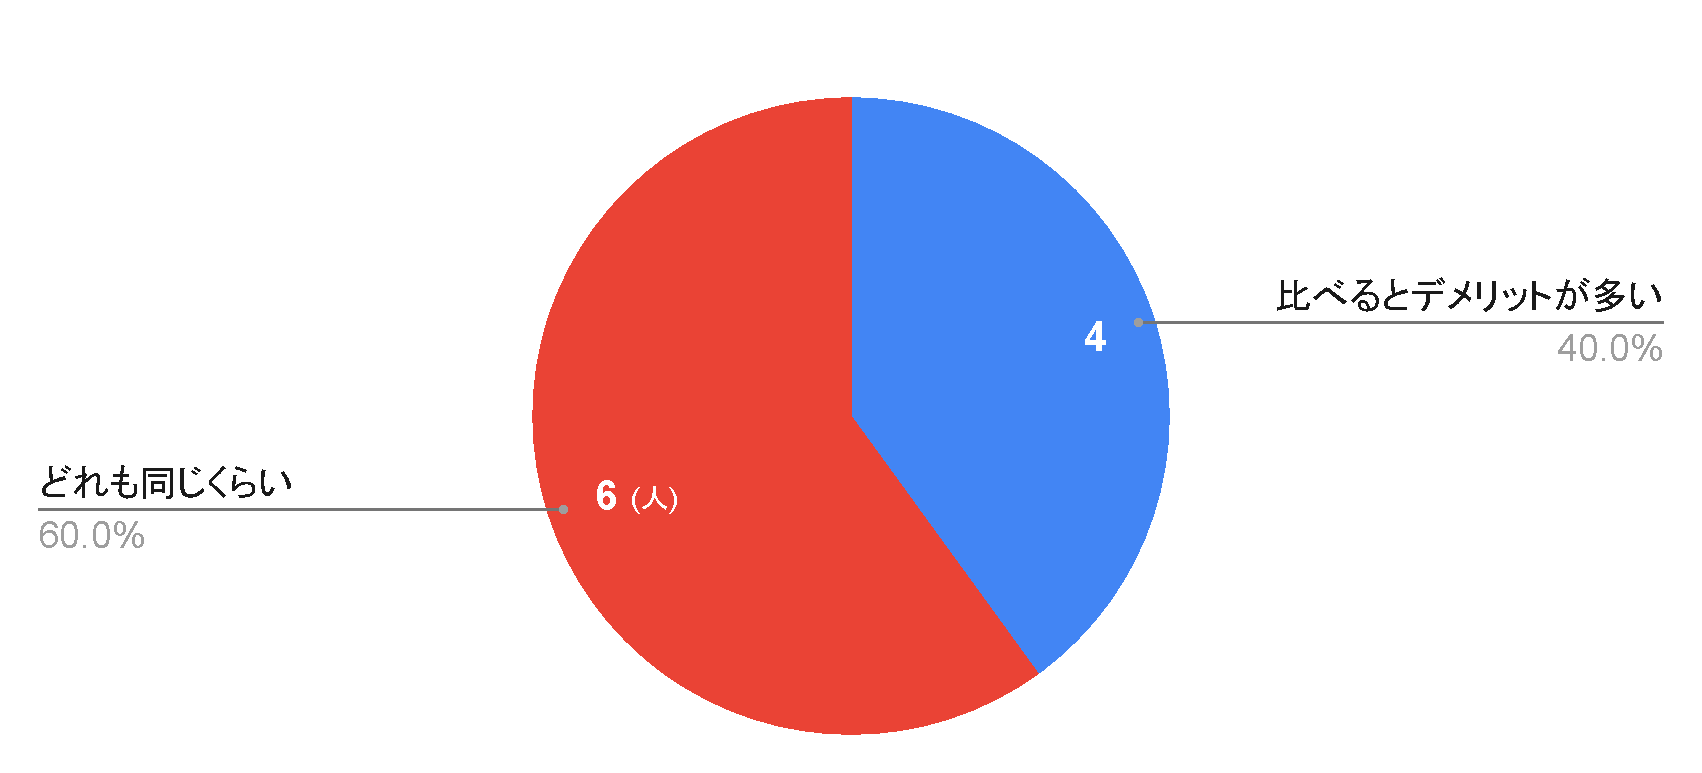
\includegraphics[keepaspectratio, scale=0.5]{比較前.pdf}
 \end{center}
 \caption{読書や映画鑑賞,スポーツ,友達と遊ぶことなど比べ,ゲームをプレイすることは利点があると思っていたか}
 \label{fig:比較前}
\end{figure}

\begin{figure}[h]
 \begin{center}
  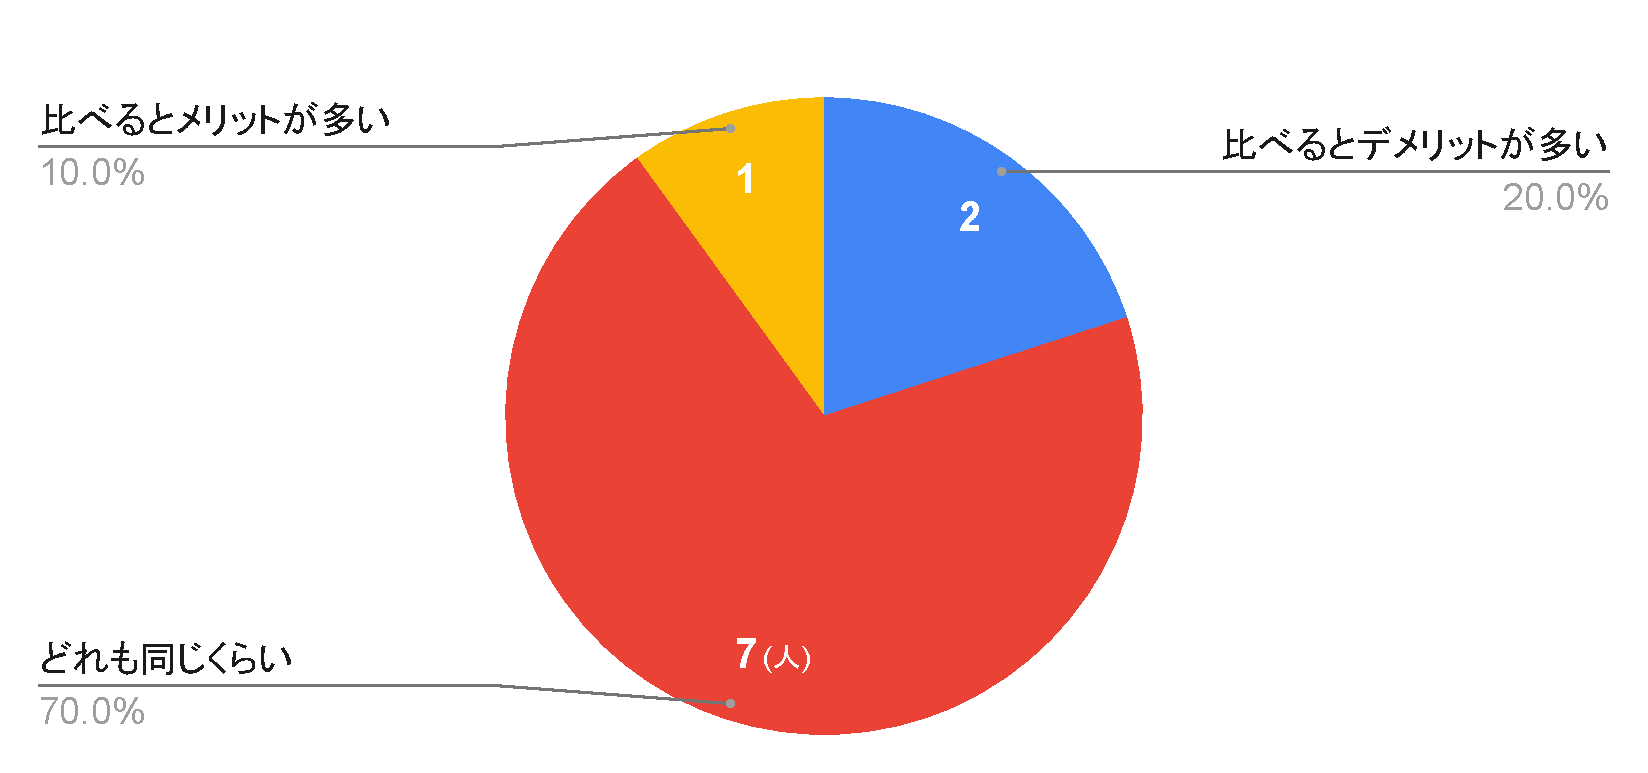
\includegraphics[keepaspectratio, scale=0.5]{比較後.pdf}
 \end{center}
 \caption{読書や映画鑑賞,スポーツ,友達と遊ぶことなど比べ,ゲームをプレイすることは利点があると思うか}
 \label{fig:比較後}
\end{figure}


\subsection{評価}
あああああああああああああ

あああああ


%5章
\section{Webサイトについて}\label{Webサイトについて}
\subsection{概要}
WebサイトはHTMLとCSSを使用して作成し,ツールとしてBootstrapを用いた.トップページに教育的メリットのタグ,教科,ゲーム一覧のボタンを設置し関連づいたゲームが表示されるようにした.構成の詳細については以下の通りである.
\subsection{ゲームの種類}
掲載したゲームは対象である小・中学生の年齢を加味し,Nintendo Switchのソフトとスマートフォンでプレイできるゲームを12個に絞った.また年齢に沿ったゲームの紹介を行う為,対象年齢を全年齢のもの9個と一部オンラインショップやバトルシーンがあり12・15歳以上になっているもの3個を掲載した.ゲーム一覧は以下の図\ref{fig:ゲーム一覧}の通りである.
教育メリットと教科の説明等

\subsection{ゲーム記事}

\vspace{1zh}
\begin{figure}[h]
\begin{center}
 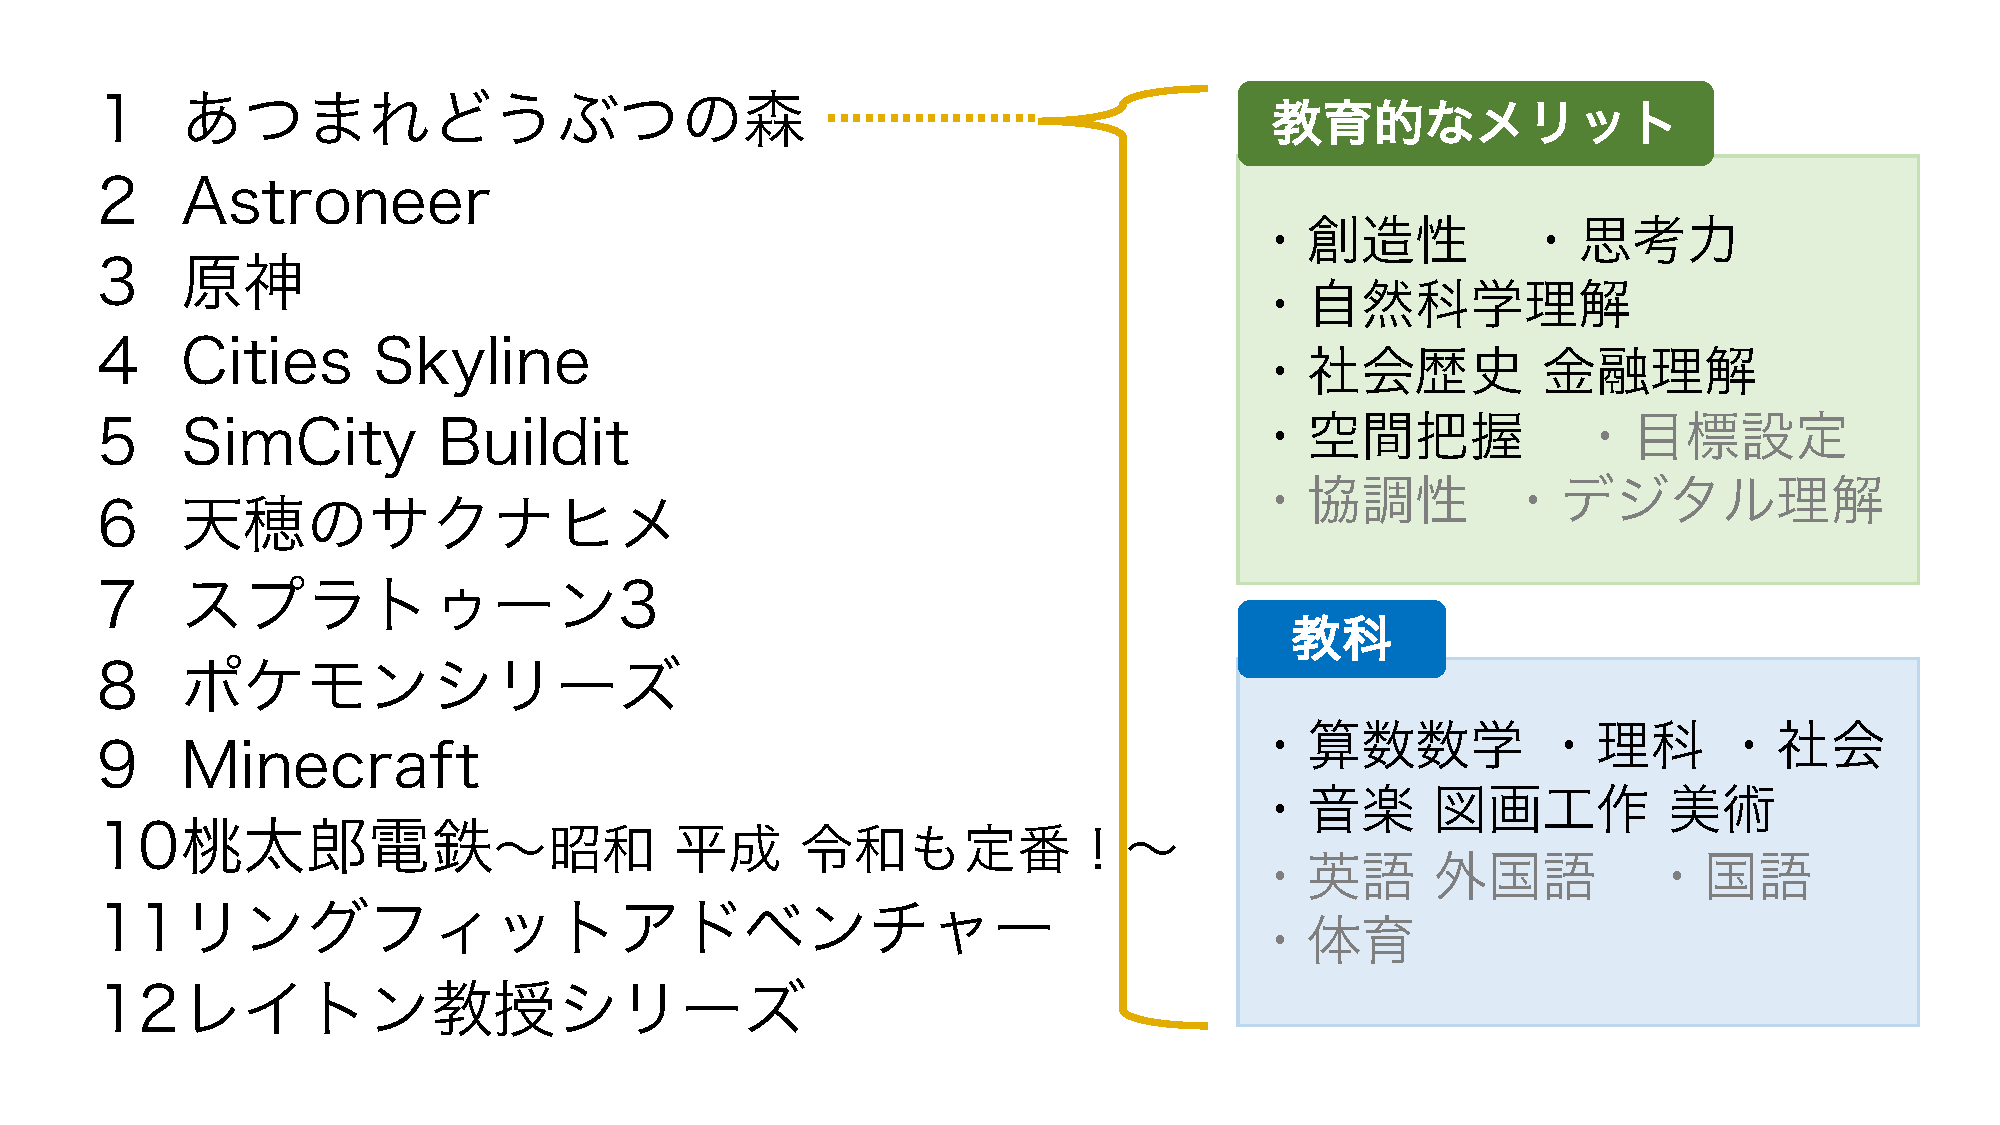
\includegraphics[clip,width=95mm,height=55mm]{games.pdf}
\end{center}
 \caption{ゲーム一覧とあつまれどうぶつの森のタグ付け例}
 \label{fig:ゲーム一覧}
\end{figure}


%6章
\section{結言}

\section{謝辞}

\begin{thebibliography}{99}
\bibitem{gameanq} ASMARQ : ``ゲームと子どもに関するアンケート調査'', \url{https://www.asmarq.co.jp/data/mr201409game/}, 2022/8/19参照
\bibitem{tvgame} 坂元 章 : ``21世紀はテレビゲーミング社会 ―娯楽主導から有効利用ヘ―'',特定非営利活動法人日本シミュレーション&ゲーミング学会, 2000年 10 巻 1 号 pp. 4-13, 2000.
\bibitem{依存症}戸部 秀之,堀田 美枝子,竹内 一夫 : ``児童生徒のインターネット,テレビゲーム依存傾向尺度の構成と,小学生から高校生にかけての依存傾向尺度値の横断的変化'',埼玉大学紀要 教育学部 Vol.59 No.2,pp.181-199,2010.
\bibitem{ゲーム脳の恐怖}森昭雄 : ``ゲーム脳の恐怖'',NHK出版,2002.
\bibitem{ゲーム脳}森昭雄 : ``IT社会と子どもの脳ーゲーム脳,ケータイ脳ー'',日本健康行動科学会 第3回学術大会公開特別公演,pp.87-95,2005.
\bibitem{ゲーム脳メディア}AllAbout : ``TVゲームをし続けるとどうなるのか? ゲーム脳の恐怖,''\url{https://allabout.co.jp/gm/gc/50643/},2002/10/9,2023/1/3参照
\bibitem{}
\end{thebibliography}

\end{document}
